\documentclass[a4paper, 12pt]{article}
\usepackage{barinov}
\begin{document}
\thispagestyle{empty}
\begin{center}
    \textit{Федеральное государственное автономное образовательное\\ учреждение высшего образования }

    \vspace{0.5ex}

        \textbf{«Московский физико-технический институт\\ (национальный исследовательский университет)»}
\end{center}

\vspace{10ex}

\begin{center}
    \vspace{13ex}

    \so{\textbf{Лабораторная работа №-.-.-}}

    \vspace{1ex}

    по курсу общей физики

    на тему:

    \textbf{\textit{<<>>}}

    \vspace{30ex}

    \begin{flushright}
        \noindent
        \textit{Работу выполнил:}\\  
        \textit{Баринов Леонид \\(группа Б02-827)}
    \end{flushright}
    \vfill
    Долгопрудный \\2019
\newpage
\setcounter{page}{1}
\fancyhead[R]{\nouppercase{\leftmark}}	
\end{center}

\section{Аннотация}
В работе будет исследовано явление дифракции Френеля и Фраунгофера на
щели, изучено
влияние дифракции на разрешающую способность оптических
инструментов.


\section{Оборудование}
\subsection*{Дифракция Френеля на щели}
Схема установки для наблюдения дифракции Френеля на щели представлена
на рис. 1. Световые лучи освещают щель $S_2$ и испытывают на ней
дифракцию. Дифракционная картина рассматривается с помощью микроскопа
М, сфокусированного на некоторую плоскость наблюдения П.

\begin{figure}[H]
    \includegraphics[width=0.8\linewidth]{1} 
    \captionsetup{justification=centering}
    \caption{Схема установки для наблюдения дифракции Френеля}
\end{figure}

Щель $S_2$ освещается параллельным пучком монохроматического света с
помощью коллиматора, образованного объективом $O_1$, и щелью $S_1$,
находящейся в его фокусе. На щель Si сфокусировано изображение
спектральной линии, выделенной из спектра ртутной лампы Л при помощи
простого монохроматора $C$, в котором используется призма прямого
зрения.

\begin{wrapfigure}{r}{0.3\linewidth}
    \vspace{-16pt}
    \includegraphics[width=\linewidth]{2}
    \captionsetup{justification=centering}
    \caption{Зоны Френеля в плоскости щели}
\end{wrapfigure}

Распределение интенсивности света в плоскости наблюдения П проще всего
рассчитывать с помощью зон Френеля (для щели их иногда называют зонами
Шустера). При освещении щели $S_2$ параллельным пучком лучей (плоская
волна) зоны Френеля представляют собой полоски,
параллельные краям щели (рис. 2). Результирующая амплитуда в точке
наблюдения определяется суперпозицией колебаний от тех зон Френеля,
которые не перекрыты створками щели. Графическое определение
результирующей амплитуды производится с помощью векторной диаграммы —
спирали Корню. Суммарная ширина $m$ зон Френеля $z_m$ определяется
соотношением:
\begin{equation}
    z_m = \sqrt{a m \lambda}
\end{equation}
где $a$ --- расстояние от щели до плоскости наблюдения (рис. 1), а
$\lambda$ --- длина волны.

Вид наблюдаемой дифракционной картины определяется числом Френеля
$\Phi$: квадрат числа Френеля 
\begin{equation}
    \Phi^2 = \frac{D}{\sqrt{a\lambda}}
\end{equation}
--- это отношение ширины щели $D$ к размеру первой зоной Френеля, т.е.
число зон Френеля, которые укладываются на ширине щели. Обратную
величину называют волновым параметром 
\begin{equation}
    p = \frac{1}{\Phi^2} = \frac{\sqrt{a\lambda}}{D}
\end{equation}

Дифракционная картина отсутствует, когда плоскость наблюдения П
совпадает с плоскостью щели: при $\Phi \rightarrow \infty$ мы имеем дело с
геометрической оптикой. При небольшом удалении от щели, когда число
Френеля $\Phi \gg 1$ (на щели укладывается огромное число зон), распределение
интенсивности света за щелью также можно получить с помощью законов
геометрической оптики (приближённо). Дифракционная картина в этом
случае наблюдается только в узкой области на границе света и тени у
краёв экрана.

При последующем небольшом удалении от щели (или изменении ширины щели
$S_2$) эти две группы дифракционных полос перемещаются практически
независимо друг от друга. Каждая из этих групп образует картину
дифракции Френеля на краю экрана. Распределение интенсивности при
дифракции света на краю экрана может быть найдено с помощью спирали
Корню.

При дальнейшем увеличении расстояния а (или уменьшении ширины щели
$S_2$)
обе системы дифракционных полос постепенно сближаются и, наконец, при
$\Phi \gtrsim 1$ накладываются друг на друга. Распределение интенсивности в
плоскости наблюдения в этом случае определяется числом зон Френеля,
укладывающихся на полуширине щели. Если это число равно то, то в поле
зрения наблюдается $n=m-1$ тёмных полос. Таким образом, по виду
дифракционной картины можно оценить число зон Френеля на полуширине
щели.

\subsection*{Дифракция Фраунгофера на щели}

\begin{wrapfigure}[13]{r}{0.3\linewidth}
    \vspace{-10pt}
    \includegraphics[width=\linewidth]{3}
    \caption{К фазовым соотношениям при дифракции Фраунгофера}
\end{wrapfigure}

Картина дифракции резко упрощается, когда ширина щели становится
значительно меньше ширины первой зоны Френеля, т.е. если 
\begin{equation}
    D \ll \sqrt{a \lambda} \quad \text{или} \quad \Phi \ll 1
\end{equation}

Это условие всегда выполняется при достаточно большом расстоянии а от
щели до плоскости наблюдения. Дифракционную картину, наблюдаемую в
этом случае, принято называть дифракцией Фраунгофера. Исследование
такой дифракционной картины заметно облегчается, потому 
что упрощаются фазовые соотношения. Это поясняет рис. 3. При
выполнении условия (4) разность хода между крайними лучами,
приходящими от щели в точку наблюдения $P$, с хорошим приближением можно
вычислять по формуле

\begin{equation}
    \Delta = r_2-r_1 \approx D \sin \Theta \approx D \cdot \Theta
\end{equation}

Здесь предполагается, что дифракционный $\Theta$ достаточно мал, так
что $\sin \Theta \approx \Theta$. Формула (5) справедлива при условии
$\delta \ll \lambda/2$. Можно показать, что это условие эквивалентно
условию (4).

Дифракцию Френеля и Фраунгофера можно наблюдать на одной и той же
установке (рис. 1). Однако при обычных размерах установки дифракция
Фраунгофера возникает только при очень узких щелях. Например, при
$a \approx 20-40\ \text{см}$ и $\lambda \approx 5\cdot 10^{-5}\
\text{см}$ получаем $D \ll 0,3\ \text{мм}$. Поскольку работать с
такими тонкими щелями неудобно, для наблюдения дифракции Фраунгофера к
схеме, изображённой на рис. 1 добавляется объектив $O_2$ (рис. 4).

\begin{figure}[H]
    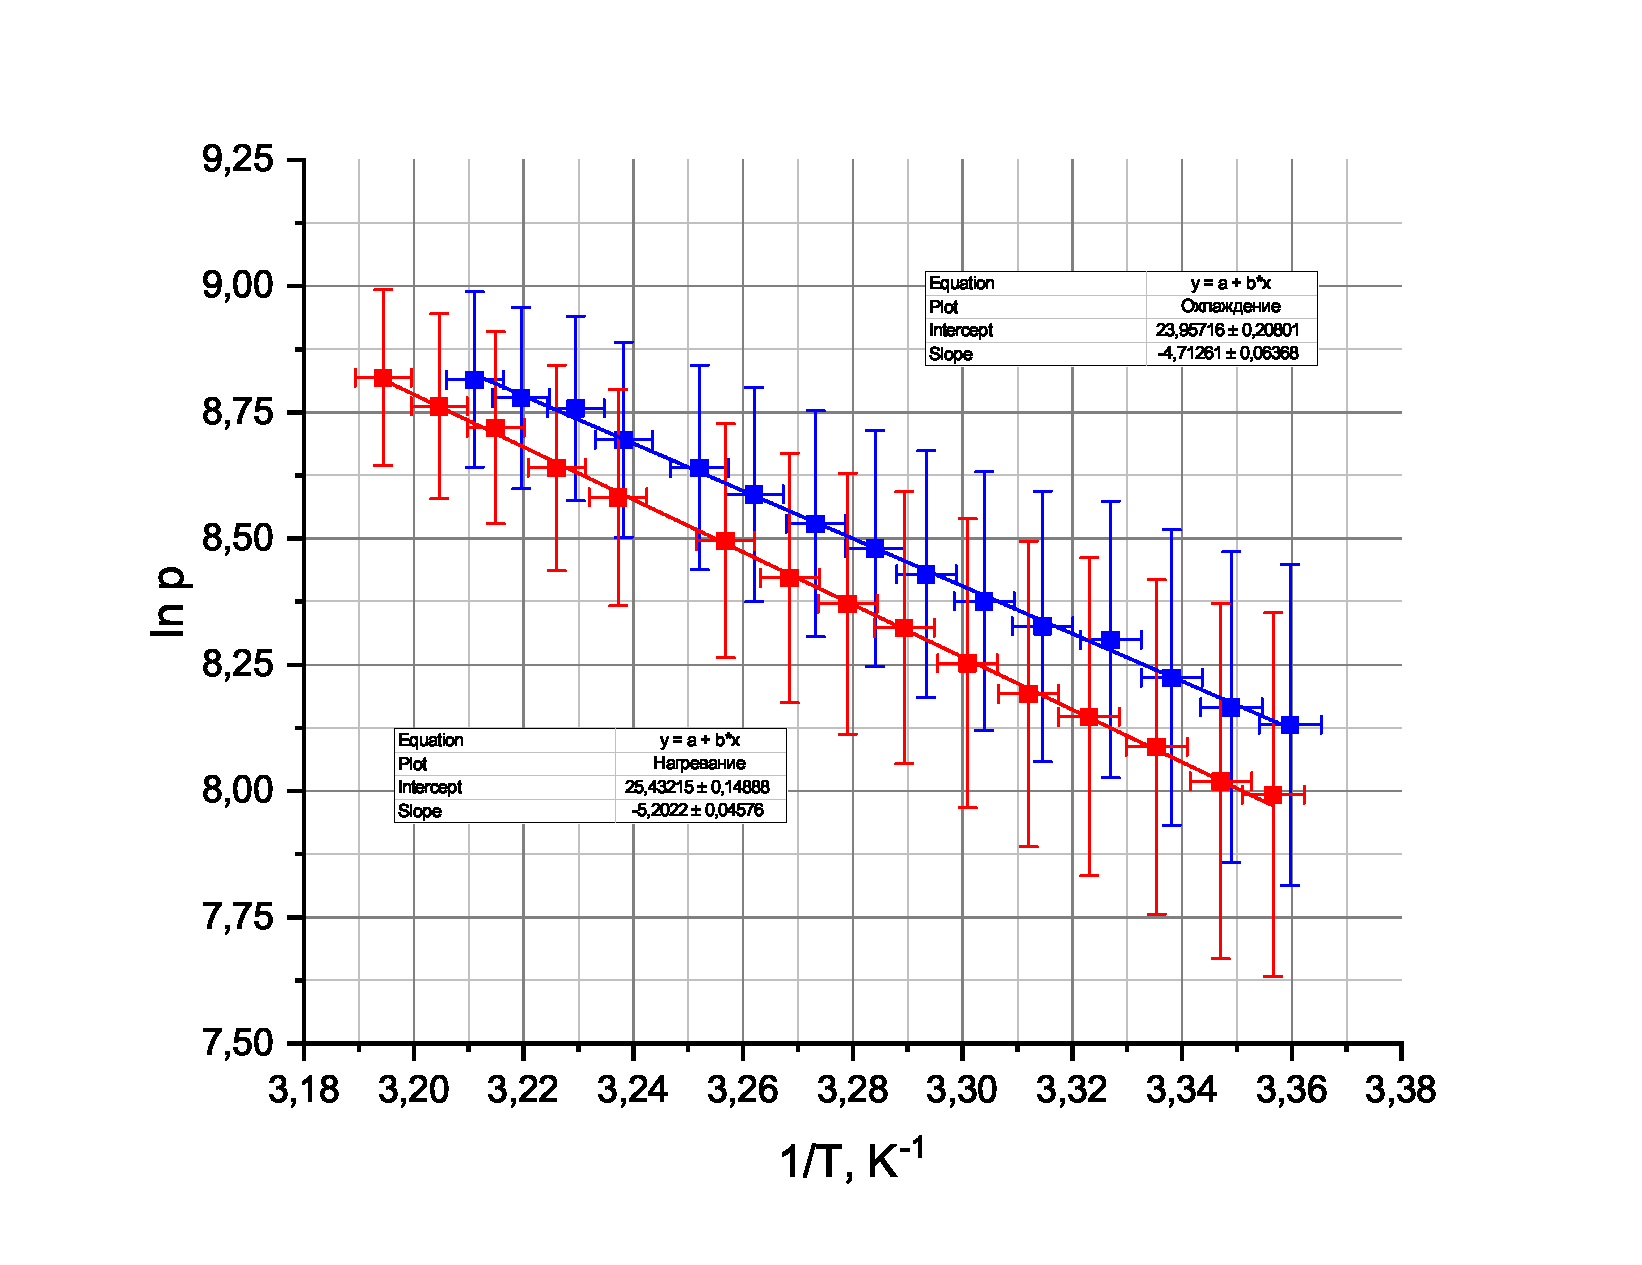
\includegraphics[width=0.8\linewidth]{4} 
    \caption{Схема установки для наблюдения дифракции Фраунгофера на
    щели}
\end{figure}

\begin{wrapfigure}{r}{0.4\linewidth}
    \vspace{-10pt}
    \includegraphics[width=\linewidth]{5}
    \caption{Распределение интенсивности при дифракции Фраунгофера на
    щели}
\end{wrapfigure}

Дифракционная картина наблюдается здесь в фокальной плоскости
объектива $O_2$. Каждому значению угла $\Theta$ соответствует в этой
плоскости точка, отстоящая от оптической оси на расстоянии 
\begin{equation}
    X = f_2 \tg \Theta = f_2 \Theta
\end{equation}

Поскольку объектив не вносит дополнительной разности хода 
между интерферирующими лучами
(таутохронизм), в его фокальной плоскости наблюдается неискажённая
дифракционная картина Фраунгофера. Эта картина соответствует
бесконечно удалённой плоскости наблюдения. Распределение интенсивности
в дифракционной картине Фраунгофера представлено на рис. 5 

Поскольку при $\Theta = 0$ разность хода между любой парой лучей равна
нулю, в центре поля зрения наблюдается дифракционный максимум (светлая
полоса). Первый минимум (первая тёмная полоса) соответствует,
очевидно, такому значению дифракционного угла $\Theta_1$, при котором в точке
наблюдения разность хода пробегает все возможные значения от нуля до
$2\pi$. Рассуждая аналогичным образом, можно определить угловую
координату $\Theta_m$ любой тёмной полосы. Для малых углов
\begin{equation}
    m\lambda = D \cdot \Theta_m
\end{equation}

Расстояние $X_m$ темной полосы от оптической оси объектива $O_2$
пропорционально фокусному расстоянию $f_2$. Из (6) и (7) следует 
\begin{equation}
    X_m = f_2 m \frac{\lambda}{D}
\end{equation}
Из (8) видно, что при малых углах минимумы эквидистантны, а расстояния
$\Delta X$ между минимумами обратно пропорциональны ширине $D$ щели
$S_2$.


\subsection*{Дифракция Фраунгофера на двух щелях}
Для наблюдения дифракции Фраунгофера на двух щелях в установке (рис.
4) следует заменить щель $S_2$ экраном Э с двумя щелями (рис. 6). При
этом для оценки влияния ширины входной щели на чёткость дифракционной
картины вместо входной щели $S_1$ следует поставить щель с
микрометрическим винтом. Два дифракционных изображения входной щели,
одно из которых образовано лучами, прошедшими через левую, а другое —
через правую щели, накладываются друг на друга.


\begin{figure}[H]
    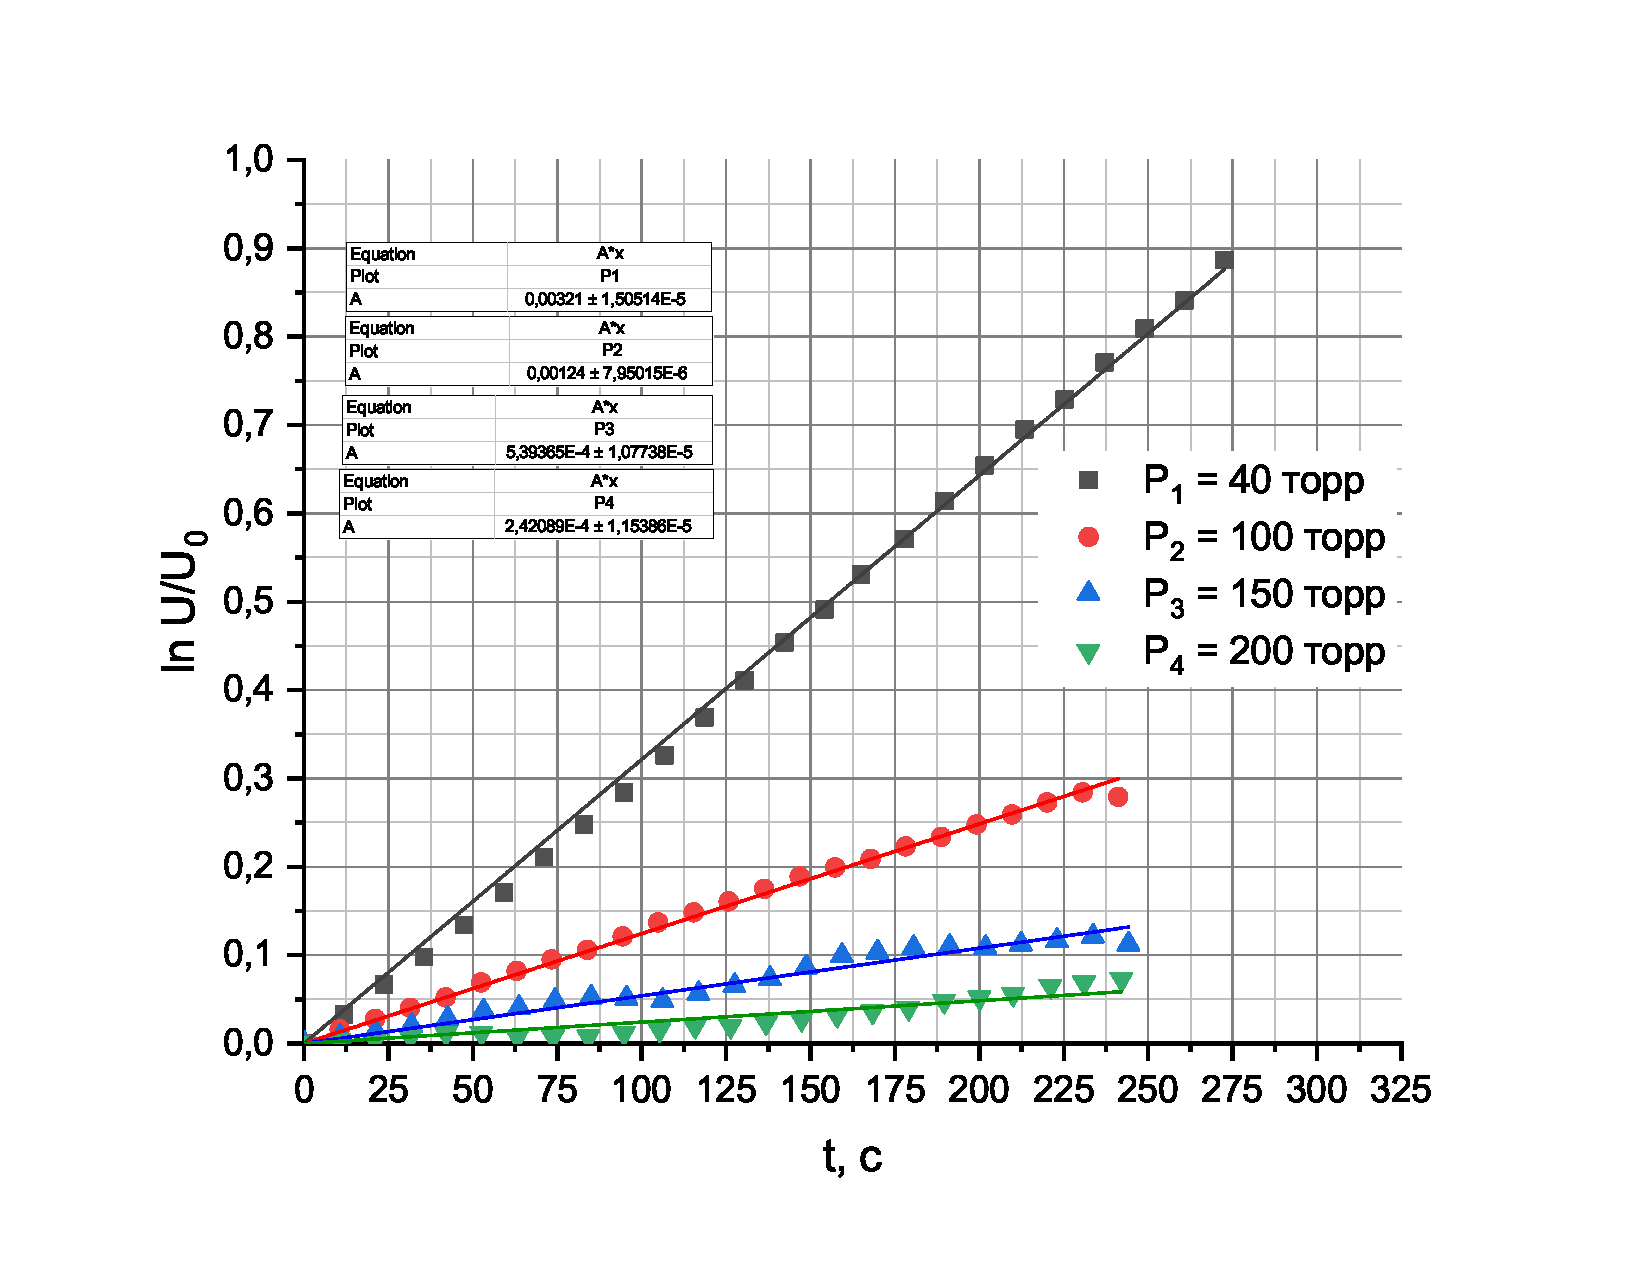
\includegraphics[width=0.9\linewidth]{6} 
    \caption{Схема установки для наблюдения дифракции Фраунгофера на
    двух щелях}
\end{figure}

Если входная щель достаточно узка, то дифракционная картина в
плоскости П (рис.~6) подобна той, что получалась при дифракции на
одной щели (рис.~4), однако теперь вся картина испещрена рядом
дополнительных узких полос. Наличие этих полос объясняется
суперпозицией световых волн, приходящих в плоскость наблюдения через
разные щели экрана Э. В центре главного дифракционного максимума (рис. 6)
располагается светлая полоса, так как при $\theta = 0$ разность хода между
этими волнами равна нулю (все лучи, приходящие в фокус объектива $O_2$,
синфазны). Светлая интерференционная полоса наблюдается и во всех
тех случаях, когда указанная разность хода равна целому числу длин
волн. Таким образом, угловая координата $\theta_m$ интерференционного
максимума $m$-го порядка определяется соотношением
\begin{equation}
    d\cdot \theta_m = m \lambda
\end{equation}
где $d$ --- расстояние между щелями.

Линейное расстояние $\delta x$ между соседними интерференционными
полосами в плоскости П равно поэтому 
\begin{equation}
    \delta x = f_2 \frac{\lambda}{d}
\end{equation}

На рис. 6 показано распределение интенсивности в фокальной плоскости
объектива $O_2$. Штриховой линией (в увеличенном масштабе) изображено
распределение интенсивности при дифракции света на одиночной щели.

Нетрудно оценить число $n$ интерференционных полос, укладывающихся в
области центрального дифракционного максимума. Согласно (8) полная
ширина главного максимума равна $2f_2 \lambda/D$, где $D$ — ширина щели, отсюда
\begin{equation}
    n = \frac{2\lambda f_2}{D} \frac{1}{\delta x} = \frac{2d}{D}
\end{equation}

При дифракции света на двух щелях чёткая система интерференционных
полос наблюдается только при достаточно узкой ширине входной щели $S$.
При увеличении её ширины интерференционная картина периодически
пропадает и появляется вновь, но полосы при этом оказываются
сильно размытыми и видны плохо. Это явление объясняется наложением
интерференционных картин от разных элементов широкой щели $S$. Первое
размытие интерференционных полос возникает при условии
\begin{equation}
    \frac{b}{f_1} = \frac{\lambda}{d}
\end{equation}
Здесь $b$ — ширина входной щели $S$ и, следовательно, $b/f_1$ — её угловая
ширина. Таким образом, по размытию интерференционной картины можно
оценить размер источника. Этот метод используется в звёздном
интерферометре при измерении угловых размеров звёзд. 

\subsection*{Влияние дифракции на разрешающую способность
оптического инструмента}
Установка, представленная на рис. 4, позволяет исследовать влияние
дифракции на разрешающую способность оптических инструментов.

Как уже было выяснено, линзы $O_1$ и $O_2$ в отсутствие щели $S_2$ создают в
плоскости П изображение щели $S_1$, и это изображение рассматривается в
микроскоп М. Таким образом, нашу установку можно рассматривать как
оптический инструмент, предназначенный для получения изображения
предмета. При этом коллиматор (щель $S_1$ и объектив $O_1$) является моделью
далёкого предмета, а объектив $O_2$ и микроскоп М составляют зрительную
трубу, наведённую на этот предмет.

\begin{figure}[H]
    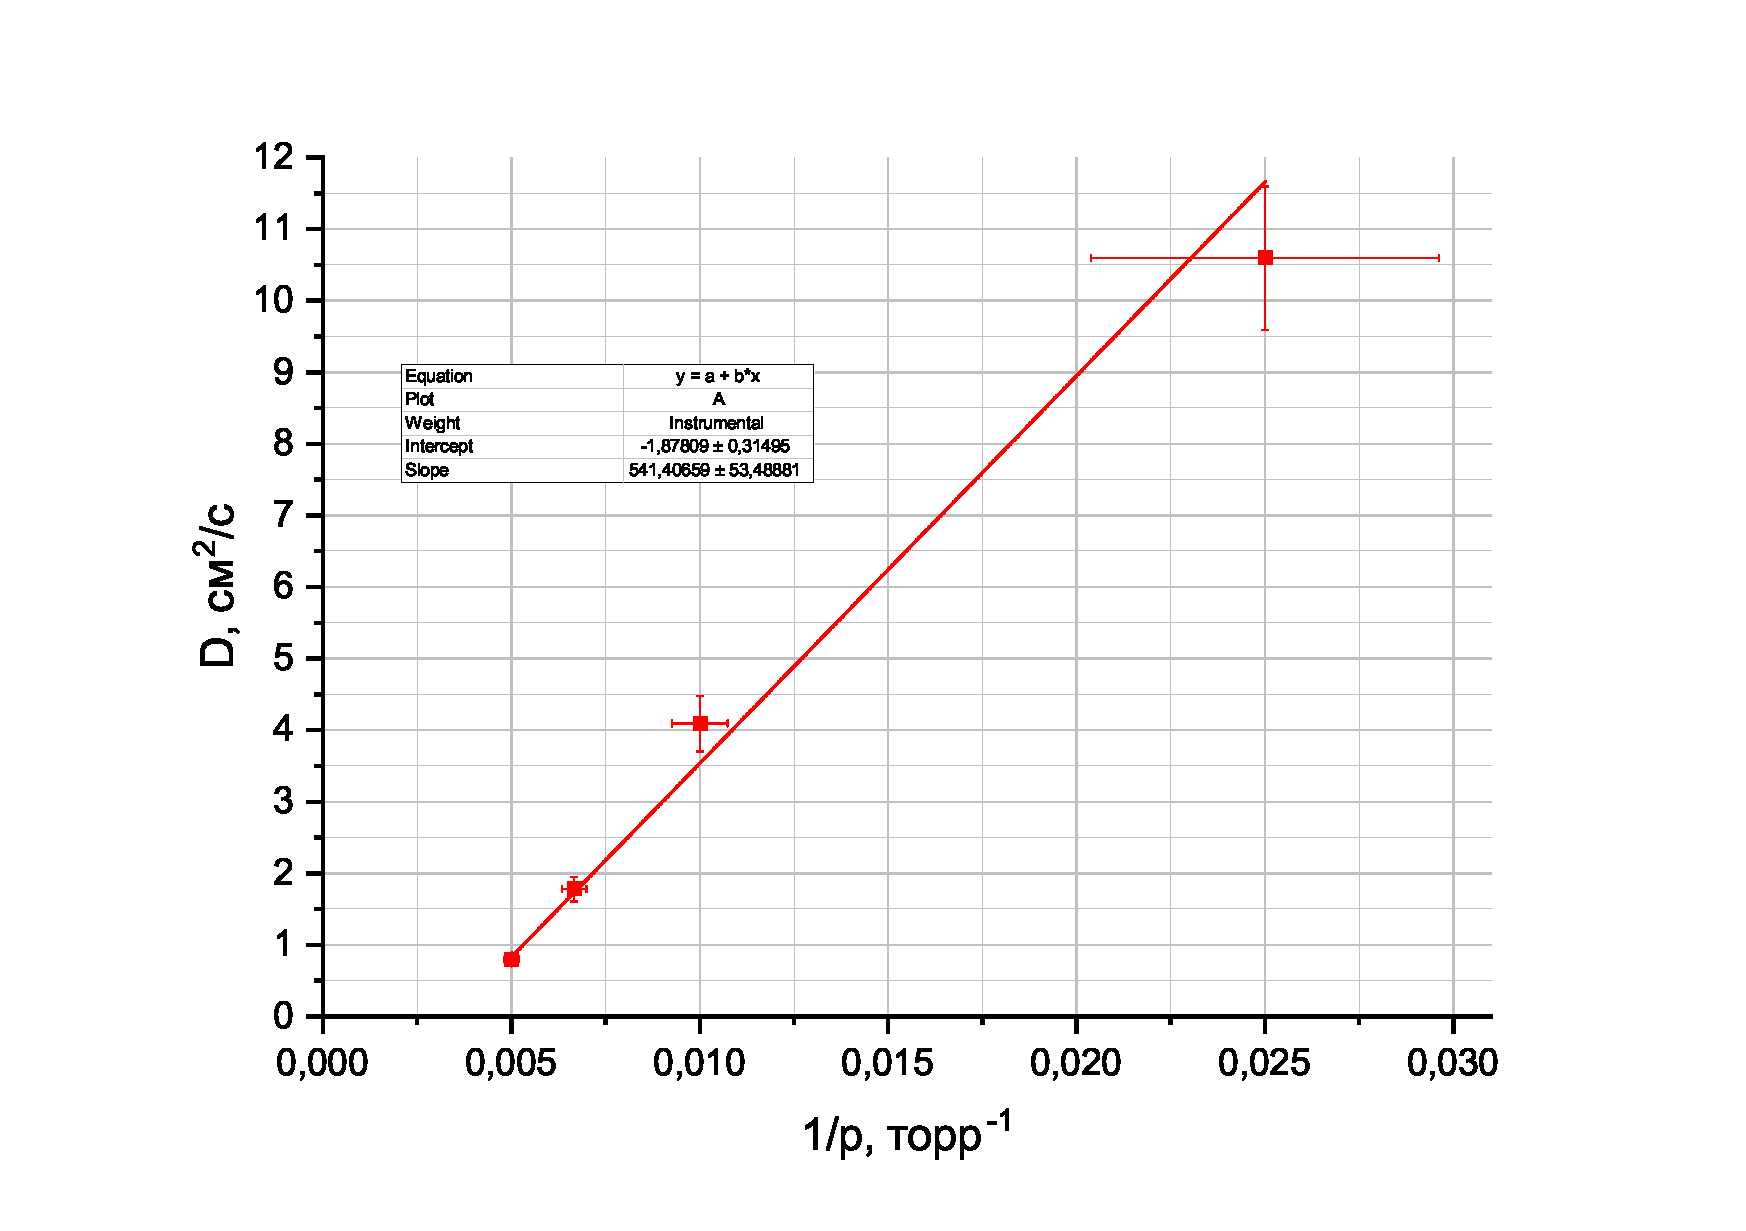
\includegraphics[width=0.9\linewidth]{7} 
    \caption{Схема установки для исследования разрешающей способности
    оптического инструмента}
\end{figure}

Если перед объективом $O_2$ зрительной трубы расположить щель $S_2$, то
изображение объекта будет искажено дифракцией на щели $S_2$. Чем меньше
ширина $D_0$ этой щели, тем сильнее искажение. Качественной
характеристикой этих искажений может служить минимальное угловое
расстояние $\phi_{\text{min}}$ между объектами (источниками), которые ещё
воспринимаются как раздельные.


Поместим вместо щели $S_1$ экран Э с двумя узкими щелями, расстояние
между которыми равно $d$(рис. 7). Тогда на щель $S_2$ будут падать два 
параллельных пучка света, составляющих между собой угол $\phi$, равный (для малых углов)
\begin{equation}
    \phi = \frac{d}{f_1}
\end{equation}

Параллельные лучи 1 и 2, проходящие через центры линз, определяют
положения изображений двойной щели. Согласно законам геометрической
оптики расстояние $l$ между изображениями щелей в плоскости П равно
\begin{equation}
    l = \phi f_2 = d \cdot \frac{f_2}{f_1}
\end{equation}
а ширина $\Delta \phi$ каждого изображения определяется дифракцией света на щели
$S_2$. Когда полуширина дифракционного изображения превышает расстояние
между изображениями, то по виду дифракционной картины трудно
определить, представляет собой источник двойную или одиночную щель.
Предельные условия, при которых ещё можно различить, имеем мы дело с
одной или двумя щелями, для разных наблюдателей различны.

\begin{wrapfigure}{4}{0.34\linewidth}
    \vspace{-10pt}
    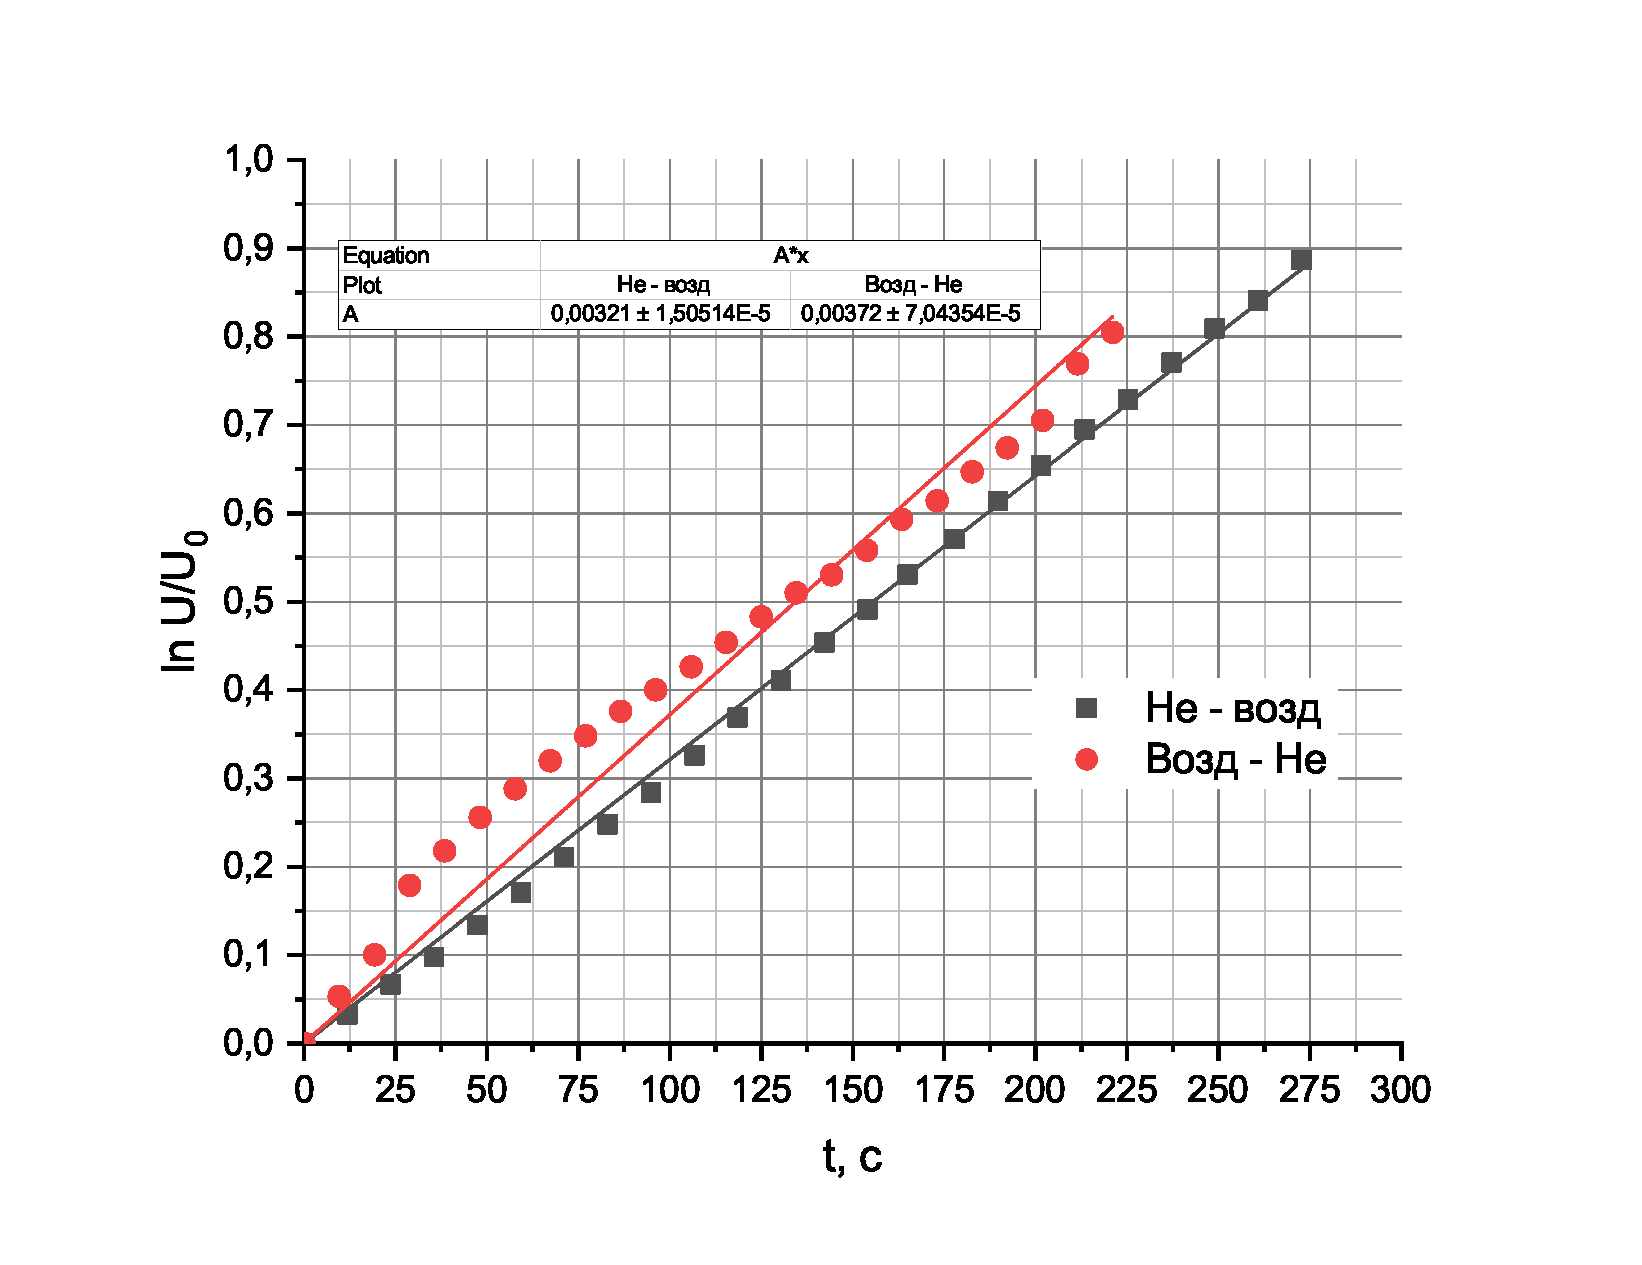
\includegraphics[width=\linewidth]{8}
    \caption{Критерий разрешения по Рэлею}
\end{wrapfigure}

Для того чтобы исключить связанный с этим произвол, пользуются обычно
критерием Рэлея, который приблизительно соответствует возможностям
визуального наблюдения: изображения считаются различимыми, когда
максимум одного дифракционного пятна совпадает с минимумом другого, а
в условиях нашей задачи — когда угловая полуширина дифракционного
изображения $\lambda$ совпадает с угловым расстоянием $\phi = l/f_2$ между
изображениями отдельных щелей (рис. 8)
\begin{equation}
    \frac{\lambda}{D_0} = \frac{l}{f_2} = \frac{d}{f_1}
\end{equation}



\section{Результаты измерений и обработка результатов}
\subsection*{Дифракция Френеля}
Ширина щели, измеренная с помощью микрометрического винта:
\[
    D_1 = (0,35 \pm 0,02)\ \text{мм}
\]

Ширина щели, измеренная с помощью микроскопа:
\[
    D_2 = (0,34 \pm 0,01)\ \text{мм}
\]


Расстояние от щели до плоскости наблюдения:
\[
    a = (2,7 \pm 0,1)\ \text{см}
\]

Длина волны желтой линии ртути:
\[
    \lambda = 578\ \text{нм}
\]


Снимем зависимость координаты микроскопа от числа $m$ наблюдаемых
темных полос. Вычислим суммарную ширину $m$ зон Френеля $z_m$ по
формуле (1).


\begin{table}[H]
\centering
\begin{tabular}{|c|c|c|c|c|c|c|}
   \hline  
$m$  & 1     & 2     & 3     & 4     & 5     & 6     \\ \hline
$a,\ \text{см}$  & 2,7   & 1,8   & 1,2   & 1     & 0,85  & 0,75  \\ \hline
$z_m,\ \text{мм}$ & 0,125 & 0,144 & 0,144 & 0,152 & 0,157 & 0,161 \\ \hline
\end{tabular}
\caption{Зависимость координаты микроскопа $z_m$ от числа $m$
наблюдаемых полос}
\end{table}

Построим график $2z_m = f(m)$

\begin{figure}[H]
    \includegraphics[width=0.9\linewidth]{9} 
    \caption{График зависимости $2z_m = f(m)$}
\end{figure}







\section{Обсуждение результатов и выводы}







\end{document}
